\chapter{Analyse der Ausgangssituation} \label{cha:ausgangssituation}
	Dieses Kapitel diskutiert die Motivation für die Abschlussarbeit, setzt klare Ziele sowie Rahmenbedingungen und erörtert den Einfluss des Java Modulsystems auf \textsc{Renew} wie auch die derzeitige Plugin-Architektur. Des Weiteren wird ein Zustand ermittelt, der als Basis für die nachfolgenden Prototypen gelten wird.

\section{Motivation}\label{sec:motivation2}
	\textsc{Renew} ist ein Petri-Netz Simulator, der von dem Arbeitsbereichs TGI/ART entwickelt wird und unterstützt das Erforschen von komplexen Systemen auf der Grundlage formaler Modelle.\newline
	Weil \textsc{Renew} in Java geschrieben ist, ist die Applikation an die Java Plattform angewiesen und muss dementsprechend den Plattformanforderungen und Richtlinien folgen. Die Anforderungen und Richtlinien einer Plattform sind nicht festgelegt und können sich ändern, besonders mit einem großen Versionssprung. Das neu eingeführte Modulsystem von Java, wird mit einem großen Versionssprung in Verbindern gebracht und setzt neue Normen und Anforderungen für die Entwicklung einer Java Applikationen. \bigbreak
	
	Es gibt mehrere Gründe warum \textsc{Renew} die Migration auf das Modulsystem durchführen sollte. Im Folgenden werden die wesentlichen Argumente, die für die Migration sprechen diskutiert.  

	\subsection{Evolution der Plugin-Architektur} \label{sub:architektur}
		Die initiale Entwicklung von \textsc{Renew} begann miteiner monolithischen Architektur. Diese erfüllte die nötigen Anforderungen, eignet sich jedoch nicht für Entwickler mit geringer Kenntnis über die Gesamtarchitektur und den darunterliegenden Konzepten. Daher wurde eine Plugin-Architektur aufgesetzt, die es ermöglichte Studenten \textsc{Renew} mit Logik innerhalb eines Plugins zu erweitern. Dieses Verfahren trägt bereits den Gedanken der Modularisierung in sich, da die Gesamtarchitektur in Bestandsteile zerlegt und miteinander entkoppelt verknüpft wird. Somit wäre die Einführung des Modulsystems von Java der nächste Schritt in Richtung erweiterbare und zusammensetzbare Systeme.

	\subsection{Parallele und Verteilte Entwicklung}\label{sub:vez}
		Die Aufteilung einer monolithischen Architektur auf eine Plugin-Architektur war ein großes Ereignis für Renew. Denn mit der Zerlegung der Gesamtarchitektur wurde die Komplexität auf die entstandenen Komponenten aufgeteilt und erlaubte eine mühelose Weiterentwicklung der Applikation über die Plugins. \bigbreak

		Obwohl die \textsc{Renew} Plugin-Architektur lange im Betrieb blieb, hatte das Plugin-System die Codebasis umorganisiert, ohne diese zu verändern. Diese führt zu altem, unverständlichem Code aus der Java 1.4 (2002) Version, mit dem viele Konzepte und Architektur Entscheidungen getroffen wurden. Nach fast 18 Jahren Betrieb altert die Codebasis, die Ideen und Konzepte für die Umsetzung ihrer Funktionalität. Besonders konfus und aufgebläht können Funktionsumsetzungen erscheinen, die heute von Java 12 in ein paar Zeilen gelöst werden können. Der zügige und rapide Wandel der Software Paradigmen und deren optimaler Einsatz in der Software Architektur ist ein Teil des Fortschritts und muss in die Planung des Lebenszyklus der Applikation mit einkalkuliert werden. \newline
		Dementsprechend ist die Modularisierung und dessen Anforderung an die Struktur und Inhalt ein wichtiges Ereignis für den \textsc{Renew} Lebenszyklus. Denn dieser erreicht wieder sein Ende und wird mit dem Modularisierungsschritt zurückgesetzt. \bigbreak

		\textsc{Renew}'s Entwicklungseinheit ist das Plugin. Diese repräsentiert ein bestimmtes Feature mit einem eigenen Lebenszyklus, wie zum Beispiel ein Formalismus, Simulator oder Fenster Management Plugin. Diese müssen Daten entgegennehmen, diese verarbeiten und wieder ausgeben. Demzufolge bündelt ein Plugin mehrere Fähigkeiten, die zusammen ein Feature verkörpern. Der wesentliche Nachteil einer Codeänderungen in einem größeren Plugin, ist das Beeinträchtigen des Gesamtverhaltens des Plugins und fordert dementsprechend ein komplettes Testszenario aller Plugin Fähigkeiten.\newline
		Mit der Einführung der Module, kann das Plugin in kleinere Einheiten zerlegt werden, die anschließend eine gekapselte Teilfunktionalität des Plugins in sich tragen und Auswirkungen der Modifikation eingrenzen. Diese sind klein, leicht änderbar, ersetzbar und besitzen einen eigenen unabhängigen Lebenszyklus. Somit verkürzt sich die Entwicklungsdauer einer Änderung innerhalb eines Plugins, da der Einfluss auf die Umgebung durch die Modulgenerzen eingeschränkt ist. Des Weiteren  bieten Module eine Möglichkeit kooperativ und parallel an einem Plugin zu arbeiten, indem die Module gegen vereinbarte Schnittstellenbeschreibungen entwickelt werden. \bigbreak

		Demnach erweitert die Modularisierung den \textsc{Renew} Kontext und erlaubt das Entwickeln von Plugins in Rahmen eines Studenten Projekts, indem Teilaufgaben eines Plugins auf Module zerlegt und parallel von Studenten bearbeitet werden können. Darüber hinaus ist das Zusammenführen der Ergebnisse eine konfliktfreie Angelegenheit und bedarf keiner kompletten Gruppenaufmerksamkeit, um die passenden Codeblöcke für die Gesamtfunktionalität auszuwählen, da es sich so gut wie keine Überschneidung in der Aufgaben Implementation bilden kann. Somit profitiert \textsc{Renew} von den kurzen Entwicklungszyklen der Module und deren unproblematischen Verknüpfungseigenschaften. 

	\subsection{Kommutative Code-Bausteine}\label{sub:cbs}
		Eine der wichtigsten Fähigkeiten eines Entwicklers, ist die Beherrschung der Komplexität. Diese führt zu sauberem, lesbarem, wartbarem Code und erweitert den Lebenszyklus einer Software um ein Vielfaches. Um diese Kompetenz zu meistern, bietet das Modulsystem von Java unterstützende Werkzeuge, die den erstellten Code organisieren und strukturieren, um ein langlebiges Ergebnis zu erzielen.\bigbreak

		Da \textsc{Renew} das Produkt vieler Abschluss-, Projekt- und Promotionsarbeiten ist, durch die die Software ihre Gestalt annimmt, gibt es diverse Beschäftigte mit eigenen Zielen und Interessen. Daher ist eine allgegenwärtige, globale Strukturanforderung, die jedem Entwickler bekannt ist und die verpflichtend eingehalten werden muss, eine erstrebenswerte Charakteristik.\bigbreak

		Die im Kapitel \ref{cha:modularisierung} vorgestellten Modul Charakteristiken beschreiben die von dem Java Modulsystem eingesetzten Richtlinien für die saubere Softwareentwicklung und erzwingen zum Teil ein Still der fein granulierten Code-Bestandteile, die kombiniert ein Softwaresystem ergeben.\newline
		Die Charakteristiken fördern den Entwickler zum Entwickeln von abgeschlossen Einheiten auf und verhindern somit das Entstehen von den sogenannten \textit{Spaghetti Code}, der funktionsübergreifende Anpassungen trifft und den Überblick über den Zusammenhang der Gesamtarchitektur unscharf erscheinen lässt. \bigbreak

		Die Module und die entsprechenden Richtlinien erschweren den \textit{Spaghetti Code}, indem Mehraufwand für die Kommunikation zwischen den Modulen erbracht werden muss und machen das unsaubere Arbeiten unattraktiv. Somit dienen Module als Grenzen für den Entwicklungsrahmen eines Features und engen den Bearbeitungs- und Betrachtungsraum für den Entwickler ein. Daraus ergibt sich ein Softwarepaket, das unabhängig von den Senior-Entwicklern verstanden, genutzt und angepasst werden kann, da der Aufbau nicht mehr in dem Wiki, Readme oder beim Entwickler selbst verankert, sondern direkt in der Codebasis integriert ist.\bigbreak

		Demzufolge profitiert \textsc{Renew} von der Modularisierung, indem sich immerfort wechselnden Akteure eine saubere Codebasis hinterlassen, die den nächsten Absolventen sowie den wissenschaftlichen Mitarbeitern viel Zeit erspart. \bigbreak

		Aus einer sauberen Umsetzung folgen saubere Code-Bausteine, die wiederverwendet werden können. Die genannten Eigenschaften der Module bringen einen wesentlichen Vorteil beim Optimieren der \textsc{Renew} Applikation, indem kontextbezogen Module ausgetauscht werden können, um ein besseres, lokales Ergebnis zu erzielen. Zum Beispiel können zielgerichtet ausgewählte Plugins für die Erfüllung einer speziellen Aufgabe, wie das Validieren von P/T-Netzen, ein besseres Ergebnis abliefern, indem ein für diesen Anwendungsfall angepasste Verarbeitungsalgorithmus angewandt wird. Dieser ist natürlich in einem Modul gekapselt und besitzt Schnittstein identisch zu seinem Vorgänger. Auf diese Weise kann eine große Anzahl an Modulen mit gleicher Funktion und unterschiedlicher Zielsetzung erstellt werden, die in einem Modulkatalog verwaltet und bei Bedarf ausgetauscht werden können.

	\subsection{Code Management}\label{sub:code_managment}
		Das Plugin Management ist ein zentrales Themengebiet von \textsc{Renew}, da Plugins geladen instanziiert und genutzt werden müssen. Diese wichtige Aufgabe übernimmt der \textit{PluginManger} innerhalb des \textit{Loader}-Plugins, der Plugins in den Klassenpfad lädt und mit den benötigten Bibliotheken ausstattet. Das Laden geschieht über den Plugin-Klassenlader, der den Code aus den gegebenen Quellen auf den Klassenpfad platziert.\bigbreak
		\begin{figure}[t]
		  \centering
		  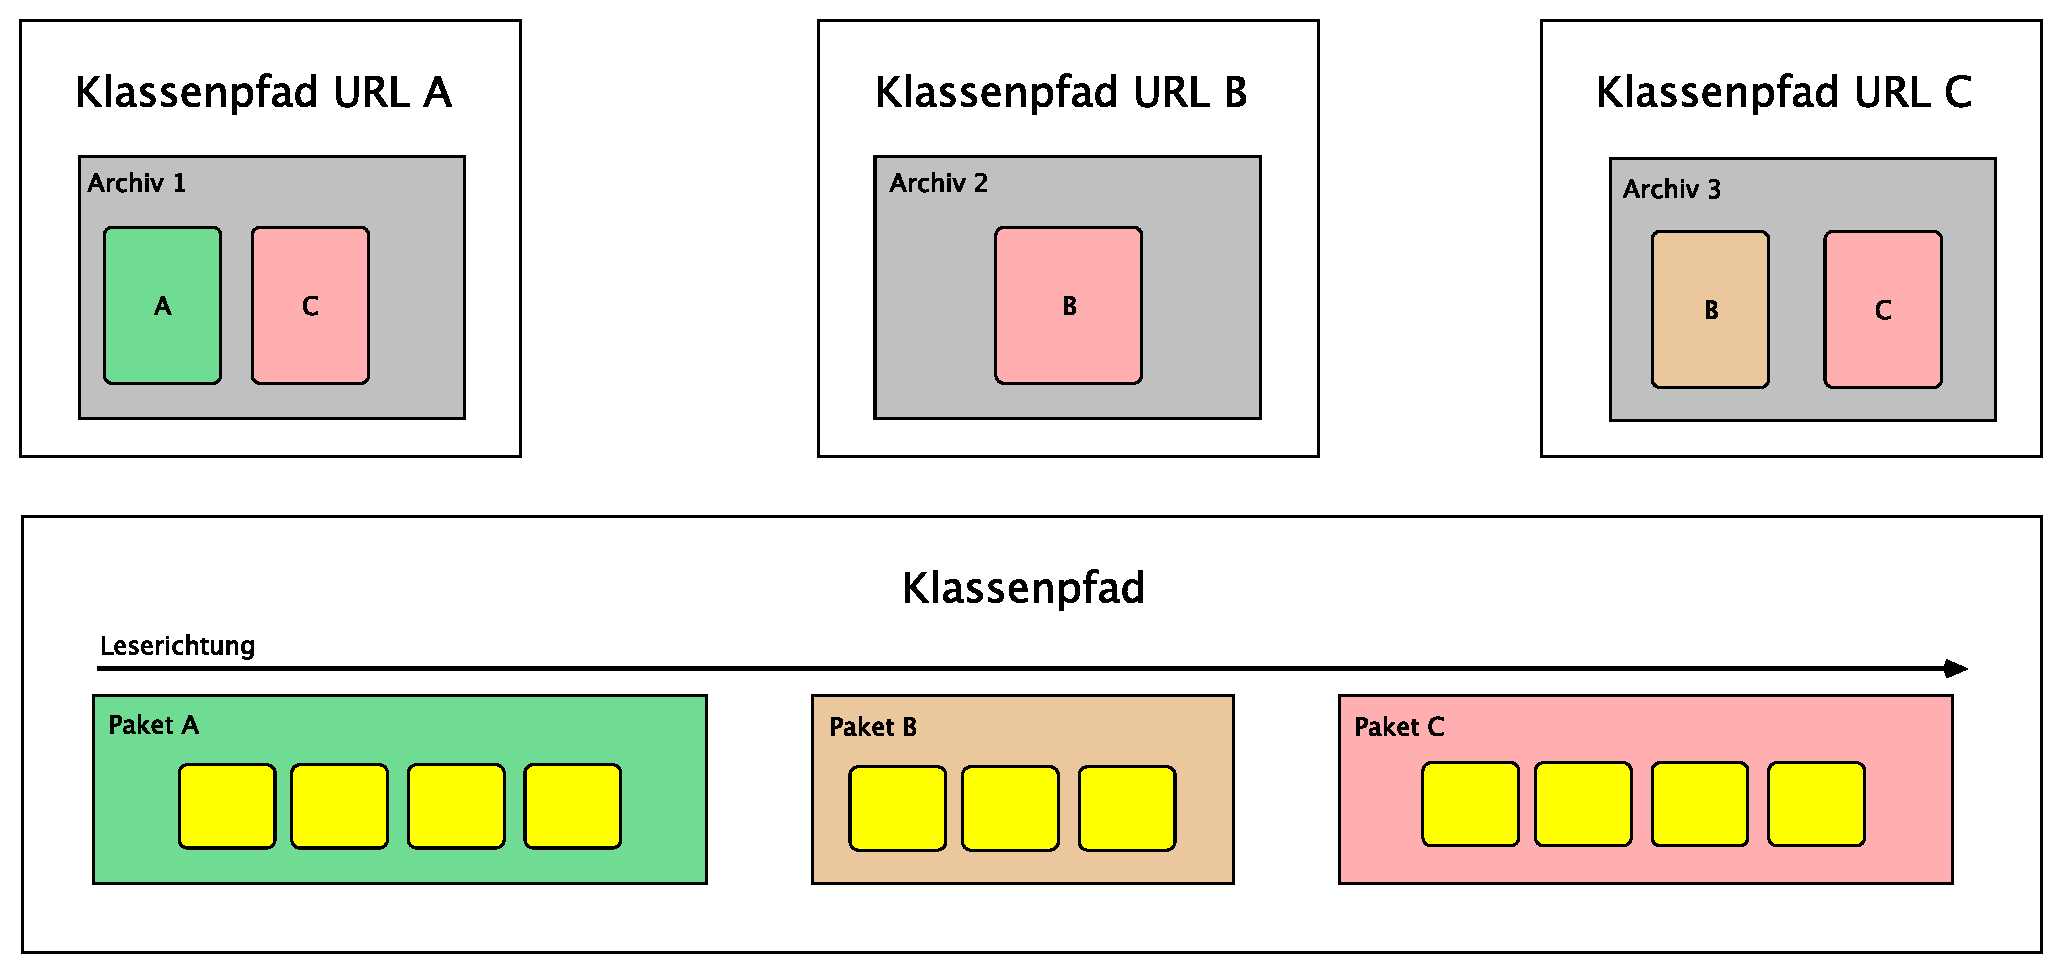
\includegraphics[width=\textwidth]{material/images/Klassenpfad.pdf}
		  \caption{Klassenpfad Suche \cite{kothagal2017modular}}
		  \label{fig:CP_Struktur}
		\end{figure}
		Der große Nachteil des Klassenpfads ist die Auflösung von Archiv Grenzen und somit auch von Plugin Grenzen. Das heißt, Java kann nicht unterscheiden aus welcher Bibliothek die Klasse stammt und muss aus diesem Grund den kompletten Klassenpfad für eine Plugin Klassenabfrage durchsuchen. Infolgedessen ist das Überwachen der Plugins auf dem Klassenpfad nur schwer möglich, da der Klassenpfad nur Informationen über die Klassen und ihre Pakete besitzt \ref{fig:CP_Struktur}. Des Weiteren ist die Zuordnung einer Klasse zu ihrer Quelle ebenso problematisch.\bigbreak

		Dieses Verfahren wurde ständig bemängelt und wird mit der Einführung des Modulsystems von Java adressiert, indem die Konfigurationsdateien \textit{module-info.java} eingeführt wurde, die der Klassen Quelle eine Identität verleiht. Demzufolge ist ein Archiv oder Verzeichnis nicht mehr ein Aussagen loser Behälter, sondern ein Objekt, das Information über seine Kennung, seinen Inhalt und seiner Kommunikationspartner besitzt.\newline
		Dies bring zwei wesentliche Vorteile für die Arbeit mit dem Plugin Code. Die erste Eigenschaft beschreibt Referenzen auf Archiv-Objekte, die die benötigten Klassen besitzen. Der Klassen werden nicht mehr von links nach rechts durchsucht \ref{fig:CP_Struktur}, wie es vorher der Fall war, sondern über das Modul mit den entsprechenden Klassen adressiert \ref{fig:MP_Struktur}.\cite{kothagal2017modular} \newline
		Das bewusste Nachschlagen nach Klassen erhöht die Performance und setzt zusätzlich das eindeutige und verantwortliche Modul für die gegebene Implementation fest. Darüber hinaus erleichtert die eindeutige Modulzuordnung das Verfolgen von unerwarteten Verhalten, wie zum Beispiel das Überdecken von Klassen von weiteren Klassen desselben Typs, die sich weiter vorne im Klassenpfad befinden.\bigbreak 
		\begin{figure}[h!]
		  \centering
		  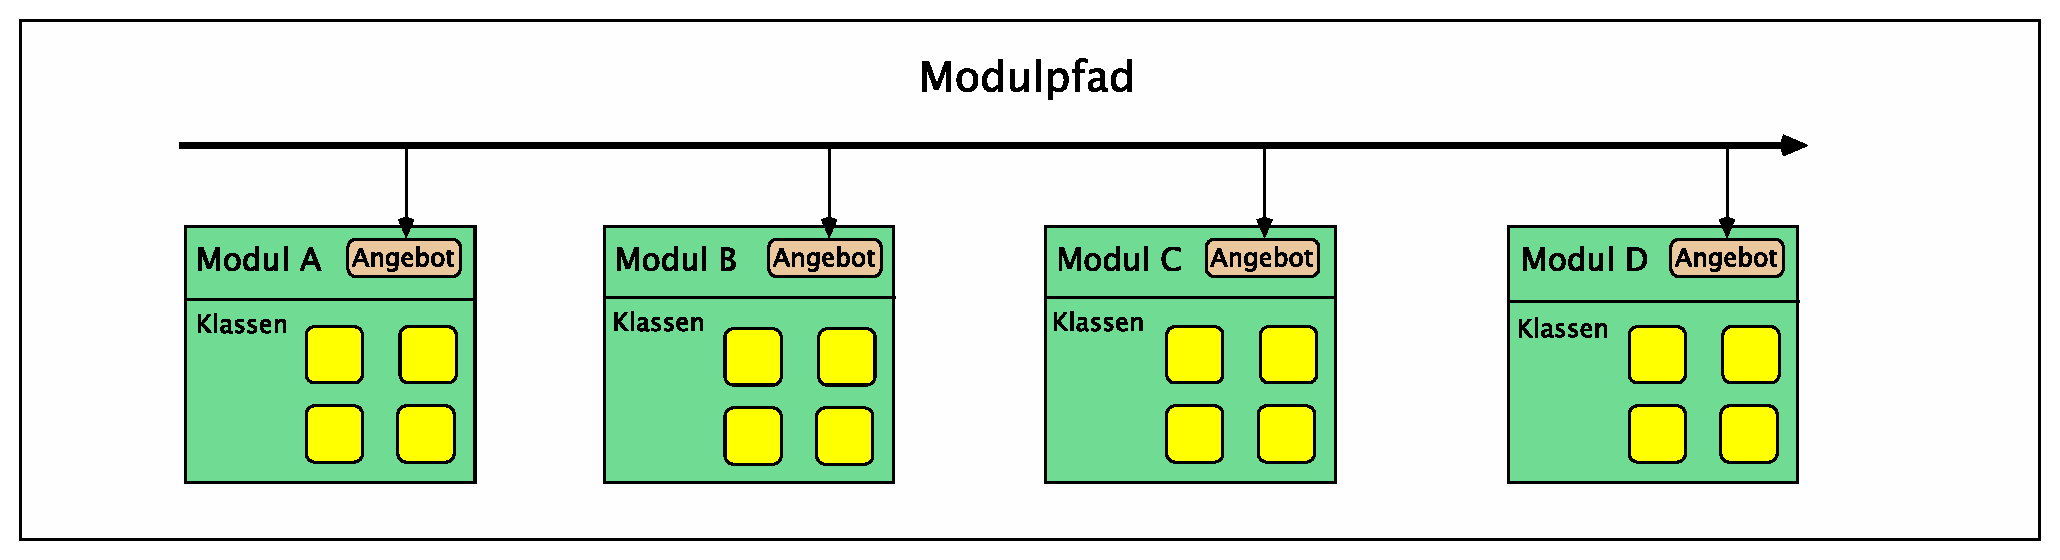
\includegraphics[width=\textwidth]{material/images/Modulpfad.pdf}
		  \caption{Modulpfad Suche}
		  \label{fig:MP_Struktur}
		\end{figure}
		Der zweite Vorteil, beschreibt das Auslesen der Modulinformation aller Module, die sich auf den Modulpfad befinden. Demzufolge können Plugins in Archive verpackt und auf dem Modulpfad wiedergefunden, analysiert und sogar bearbeitet werden. Somit bring Java ein neues Instrument zum Verwalten der Codebasis von modularisierten Anwendungen, die dem Nutzer bei Bedarf die internen Bausteine präsentieren lässt.\bigbreak

		\textsc{Renew} kann mithilfe der neuen API des Modulsystems die Verwaltung der Plugins erweitern, indem geladenen Plugins direkt angesprochen und manipuliert werden. Zum Beispiel könnten auserwählte Plugins nur für bestimmte Nutzer oder Modi ihre Funktionalität anbieten oder eine angenehme Visualisierung der laufenden Plugins und dazugehörige Funktionalitäten dem Nutzer präsentieren. Des Weiteren ist die performante Suche nach Klassen in einem dynamischen System wie \textsc{Renew}, eine erstrebenswerte Qualität.  \newline
		Im folgenden Kapitel der Auswirkungen \ref{sec:auswirkung} wird auf die \textit{Modulschicht} eingegangen, die das zielorientierte Laden nur notwendiger Module und somit nur notwendiger Plugins ermöglicht.

	\subsection{Abgeschlossene Laufzeitabbildung} \label{sub:laufzeit_images}
		Für die Nutzung von Java Applikationen ist immer eine installierte Laufzeitumgebung notwendig, die Versionskompatibel mit der entsprechenden Applikation sein muss. Dementsprechend muss Java installiert und eingerichtet werden bevor der Code ausgeführt werden kann. Für große Serveranwendungen ist der Aufwand gerechtfertigt, da sie unikale, langlebige und komplexe Gebilde darstellen. Für Anwendungen, die kleiner sind und dynamisch zwischen Hardwareknoten verteilt werden müssen, ist das manuelle Anlegen der Laufzeitumgebung eine mühselige und fehleranfällige Aufgabe. \newline
		Das Modulsystem von Java hat diese Herausforderung mithilfe der \textit{Laufzeitabbildung} adressiert. Die \textit{Laufzeitabbildung} besteht aus einer Verzeichnisstruktur, die alle notwendigen Komponenten für den Betrieb der Applikation besitzt. Dazu zählen Module, Skripte, native Bibliotheken, Konfigurationen, Dokumentationen sowie Lizenzbedingungen und sogar Sicherheitsmechanismen zum Validieren der Komponenten sind vorgesehen. Die generierten \textit{Laufzeitabbildungen} sind in sich Abgeschlossen und können einfach auf beliebig viele Hardwareknoten automatisiert verteilt und ausgeführt werden, ohne zusätzliche Justierung der Software Umgebung. \bigbreak
		Die Eigenschaft der Abgeschlossenheit der \textit{Laufzeitabbildung}, kann von \textsc{Renew} aufgegriffen und genutzt werden, um ausgewählte Plugin Gruppen horizontal nach Belieben zu skalieren. Zusätzlich hält die \textit{Laufzeitabbildung} nur notwendige Java sowie Benutzer erstellte Module, die bestens für die Ausführung der Applikation aufeinander abgestimmt werden. Infolgedessen kann das modularisierte \textsc{Renew} auf optimale Ausführungsgeschwindigkeiten zählen. 

	\subsection{Integration in moderne Technologien} \label{sub:moderner_zustand}
		% Ziel
		Der zeitgemäße Zustand einer Applikation ist ein Zeichen hoher Qualität und reflektiert enorme Ansprüche an den Betrieb der Applikation. Diese kann geschäftskritische Qualitäten tragen, die den marktführenden Vorteil bringt und der Konkurrenz ein Schritt voraus ist. Um den Vorsprung zu sichern, ist eine vorausschauende Flexibilität gefragt. Mithilfe dessen die Applikation in der Lage ist, mit minimalem Aufwand, an die führenden Technologien anzuknüpfen.

		% Trends 
		Die aktuell führenden Trends beschäftigen sich mit der verteilten und wiederverwendbaren Softwareumsetzungen, die ständig an Komplexität gewinnen und trotzdem leicht beherrschbar bleiben muss. Diese beschreiben Ansätze wie gewisse Ziele erreicht werden können und setzen Grundvoraussetzungen zum Erreichen dieser Ziele. Dementsprechend muss \textsc{Renew} bestimmte Grundvoraussetzungen erfüllen, um die Vorteile der Trends zu Nutzen und den Schritt mit dem Fortschritt zu halten.  \bigbreak

		% Docker  
		Zum Beispiel wäre die Docker Umgebung für \textsc{Renew} eine willkommene Erweiterung, mit der interne Bestandsteile distributiv betrieben werden können. Somit wäre die Ausführung von \textsc{Renew} nicht mehr an eine Maschine gebunden und kann bei Bedarf horizontal skaliert werden. Im Folgenden stellt sich die Frage: Welche internen Strukturen von \textsc{Renew} müssen individuell behandelt und anschließend kooperativ zusammengeführt werden. Auf diese Frage gibt es keine pauschale Antwort, jedoch ist es klar, dass die Plugins von \textsc{Renew} feingranular betrachtet werden müssen, um sich ein Bild der Verarbeitungskette zu erstellen und diese den Bedürfnissen anzupassen. \bigbreak

		% Microservice  
		\textsc{Renew} auf verschieden Hardwareknoten zu verteilen ist nur der erste Schritt der distributiven Ausführung. Es fehlt die Koordination zwischen den Knoten, die die Verarbeitung koordinieren und die Ergebnisse zusammenfassen. Somit gibt es eine weitere Technologie, die sich dieser Aufgabenstellung widmet: Der Mikroservice Architekturansatz, der sich um die Koordination und das Zusammenspiel von Applikationsschwärmen kümmert. \bigbreak

		% Fazit 	
		Mithilfe der Mikroservicearchitektur und der Docker-Umgebung wäre die distributive Ausführung von \textsc{Renew} erreichbar, doch zuerst muss \textsc{Renew} den aktuellen Stand der Technologie entsprechen und demzufolge das Modulsystem von Java integrieren.  		
		
\section{Anforderungsanalyse} 
	Indem der Java-JDK mit der neunten Version von Java modularisiert wurde, ändern sich die grundsätzlichen Funktionsrichtlinien der Plattform, die Konsequenzen für bestehende Systeme mit sich bringen. Denn das Modulsystem von Java führt eine obligatorische Kapselung der Code-Komponenten ein, die über erweiterte Sicherheitsmechanismen verfügen und nur über explizite Schnittstellen geladen und angesprochen werden können.\newline 
	Diese Abschlussarbeit beschäftigt sich mit der Untersuchung von Anforderungen der modularisierten Java Plattform, sowie dem entsprechenden Aufwand für das Anpassen bestehender Systeme. Darüber hinaus sollen die neu eingeführten Java Konzepte für den Einsatz im Rahmen der dynamischen Systeme untersucht werden.\newline
	Für die Umsetzung muss ein grundlegendes Migrationsverfahren erarbeitet und angewandt werden, welches eine Migration auf das Modulsystem von Java ermöglicht. Da die Migration bestehender Systeme nicht in einem Schritt durchgeführt werden kann, müssen Charakteristika für Module formuliert werden, um bestehende Systemelemente innerhalb einer ausgereiften Software mit den entsprechenden Eigenschaften zu erweitern.\newline
	Jede kleine Änderung in einem komplexen System bringt große Risiken mit sich, die das saubere Arbeiten der Software infrage gestellt. Daher ist der Übergang auf das Modulsystem von Java mit Unsicherheit verbunden, zumal es Zeit kostet, im Code verankertes Geschäftswissen umstrukturiert und keine sichtbare Softwareerweiterung für den Endkunden darstellt. Demnach liegen die Schwerpunkte der Migration in der Konsistenz der gegebenen Software im neuen Kontext, dem Mehrwert sowie in dem Aufwand der Umsetzung. \newline
	Die Erarbeitung der neu eingeführten Java Konzepte muss den Mehrwert für den Einsatz im dynamischen System abbilden und einen möglichen Einsatz darstellen.

	Um die gegebenen Anforderungen an eine Applikation zu stellen, bedarf es einer passenden Projektstruktur und Umsetzungswerkzeuge, die eine Modulmenge kompilieren und verpacken. Zu diesem Zweck soll das Java basierte Gradle Werkzeug eingeführt werden, das eine kompakte und mächtige Ausdrucksform für das Erstellen von Softwaresystemen Entwicklungsumgebung unabhängig anbietet. \bigbreak

	Für die Umsetzung der erarbeiteten Konzepte steht der \textsc{Renew} Simulator und das \textsc{Mulan} Rahmenwerk zur Verfügung, die in dieser Abschlussarbeit Migrationsszenarien erleben.\newline 
	Das erste Szenario soll eine kontinuierliche Migration einer Software auf das Modulsystem modellieren. Im Gegensatz dazu wird im zweiten Szenario alt Software auf eine modularisierte Codebasis aufgesetzt und der parallele Betrieb begutachtet. 

\section{Anforderungsspezifikation} 
	Für den Anwendungskontext der Modularisierung einer größeren Anwendung steht \textsc{Renew} und \textsc{Mulan} zur Verfügung, jedoch übersteigern eine vollwertige Modularisierung von \textsc{Renew} und \textsc{Mulan} den Zeitrahmen dieser Abschlussarbeit, da die Umstellung jedes einzelnen Plugins auf organisierte Modulverbände eine zeitintensive Aufgabe verkörpert. Jedes einzelne Plugin muss analysiert, reorganisiert, auf Module zerlegt und bestens miteinander verzahnt werden. Darüber hinaus müssen die entstandenen Module mit allen gegenwärtigen Plugins abgestimmt werden, da das Plugin Modulverband generell andere Schnittstellen anbieten wird. \bigbreak
	Dementsprechend wird die Modularisierung auf einzelne Plugins reduziert, die für die Darstellung der UI sowie die grundsätzliche darunterliegende Logik zuständig sind. Um die Kommunikation im bestehenden System zu garantieren, behalten die entstandenen modularisierten Plugins ihre Schnittstellen. Infolgedessen wird die Funktionalität aller Plugins nicht beeinträchtigt und garantiert dem Gesamtsystem einen nahtlosen Übergang auf den Modulpfad. Hierfür werden die Plugin Module mit den entsprechenden Konfigurationsdateien erweitert und mit den notwendigen Plugins verzahnt. In der Konsequenz wird die Umsetzung nur die minimalen Anforderungen des Modulsystems realisieren und das Zerlegen der internen Struktur der Plugins aus der Sicht lassen, obwohl es ein wünschenswerter Schritt in Richtung der Modularisierung wäre. \newline 
	Trotz allem müssen die Plugin Projekte von \textsc{Renew} zusätzliche Module unterstützen und die Möglichkeit bieten, \textsc{Renew} zu erweitern, um weitere Module innerhalb eines Plugins erstellen zu können. Dafür benötigen alle Plugins eine neue Projektstruktur, die das gewünschte Verhalten umsetzt und die empfohlene Modulorganisation unterstützt. Dieses trägt die Maven konforme Projektstruktur, die Java Klassen, Ressourcen und sonstige Artefakte nach einem standardisierten Muster verwaltet.\newline
	Für den Einsatz von neu eingeführten Java Konzepten wird ein Grundriss aufgezogen, der eine möglichen Umsetzung der dynamischen Plugin-Verwaltung anbietet. \bigbreak

	Des Weiteren muss die Konfiguration des Projektes von der Entwicklungsumgebung gelöst werden, um den Entwickler nicht in seinem Arbeitsablauf einzuschränken und die Entwicklungsumgebung seiner Wahl zu nutzen zu dürfen. Dazu soll die existierende Ant Umgebung mit Gradle ersetzt werden. Diese erleichtert das Verwalten sowie Verpacken der Software und verspricht zusätzlich eine kohärente Arbeitsweise mit dem Modulsystem von Java, indem das Verwalten der Modulabhängigkeiten sich in beiden Systemen widerspiegeln. Diese Eigenschaft soll auf die modularisierte Version von \textsc{Renew} angewandt und evaluiert werden. \bigbreak

	Da der \textsc{Renew} Simulator von verschiedenen Abschlussarbeiten beleuchtet und erweitert wird, beinhaltete die Applikation verschiedene Techniken der Softwareentwicklung, wie zum Beispiel das Generieren von Java Klassen mit dem \textit{JavaCC} Compiler. Dementsprechend existieren ältere Verfahren innerhalb von \textsc{Renew}, die sorgfältig auf Kompatibilität mit der neuen Umgebung untersucht und migriert oder ersetzt werden müssen. \bigbreak
	Das Aufbereiten der Grundlagen sowie der Ausgangssituation sind essenzielle Schritte einer Migration, da diese das Fundament für die Planung und Umsetzung legen. Zusätzlich leitet die Ausgangssituation das Migrationsszenario, das eine beispielhafte Schrittweise Migration oder Integration demonstriert und evaluiert.\bigbreak

\section{Auswirkung von Gradle und JPMS auf \textsc{Renew}} \label{sec:auswirkung}
	Die Folgeerscheinung der Modularisierung unterbindet zahlreiche Entwicklungsschwächen, wie die \textit{Codeorganisation}, \textit{Zyklen}, \textit{Split Packages} und antiquierte API's. Diese sollen mit der Migration auf das Modulsystem von Java aufgelöst, reorganisiert und nachgerüstet werden, um einen kompilierfähigen Zustand erreichen zu können.

	\subsection{Projektstruktur} \label{sub:projektstrukutr}
		Das Plugin System von \textsc{Renew} besteht aus einer großen Anzahl an Plugins, die Zweckorienttier kombiniert werden können. Demnach besteht bereits ein Organisationsaufwand, der mit jeder Plugin Kombination wächst. \bigbreak

		Zu den bestehenden Organisationsaufwand wird eine neue Ebene der Administration eingeführt, nämlich die Ebene der Module. Diese zerlegen Aufgabenmengen aus einer Code-Struktur in mehrere Code-Bausteine, die infolgedessen innerhalb eines Plugins disjunkt verwaltet werden müssen.\newline
		Da die Kombination aus Plugins und Modulen ausschlaggebend für die \textsc{Renew} Funktionalität ist, muss eine passende Projektorganisation eingerichtet werden, die jedem Plugin die Möglichkeit bietet, zusätzliche Module mit dem Quell-Code, den Ressourcen sowie den Tests anzulegen.\bigbreak

		Des Weiteren spielt die Paketorganisation eine zunehmend stärkere Rolle im Modulsystem von Java, denn eine Überschneidung eines Paketnamens mit anderen Bibliotheken im System ist ausgeschlossen und muss dementsprechend einen global eindeutigen Namen besitzen. \newline
		Die Einschränkung in der Namensgebung und Code Organisation ist für \textsc{Renew} eine substantielle Änderung. Die Plugins wurden von unterschiedlichen Entwicklern zu unterschiedlichen Zeitpunkten entwickelt, ohne eine einheitliche Struktur Plugin übergreifend einzuhalten. Daraus folgt eine wilde Ressourcen- und Java Fremdcode Allokation, die das Lesen, Analysieren und bearbeiten der Plugins schwierig gestaltet. Zum Beispiel befinden sich gewisse Ressourcen im Plugin Wurzelverzeichnis unter \textit{tools}, \textit{samples}, \textit{ontology} und andere direkt im Java Source-Code unter \textit{src/**/*.(gif|jj|rnw|sns|vm)}. Der Aufbau führt zu der Frage, wie kompatibel ist das Ressourcenlayout mit dem Modulsystem von Java. Denn Ressourcen werden im Modulsystem von Java genauso wie die Java Klassen innerhalb eines Modulpakets gekapselt und verwaltet. Demzufolge kann das Paket \textit{samples} nur einmal in einer Modulmenge existieren, da das Modul global den kompletten Namensraum für sich und seine Ressourcen allokiert. \bigbreak 

		Das Problem der Ressourcenorganisation, kann mithilfe des \textit{META-INF} Verzeichnis gelöst werden, denn das \textit{META-INF} Verzeichnis ist ein besonderes Verzeichnis, das nicht als ein Klassenpaket interpretiert wird und dementsprechend keinen ausführbaren Code enthält. Demzufolge können namensgleiche Ressourcen Verzeichnisstrukturen in unterschiedlichen Modulen denselben Namensraum besetzen und alle benötigten Ressourcen wie Konfigurationsdateien, Bilder und komplexe Darstellungsobjekte enthalten.\bigbreak

	\subsection{Split Packages}
		Im Kapitel \ref{sub:code_managment}  wurde die neue Klassensuche innerhalb des Modulsystems von Java thematisiert. Die Klassensuche ordnet jedes Klassenpaket eindeutig einem Modul zu, um den Klassenpfad durch eine Struktur zu erweitern, die sicher, schnell und eindeutig ist. Für \textsc{Renew} ist die Voraussetzung der eindeutigen Paketbenennung noch nicht erfüllt. Denn \textsc{Renew} besteht aus Plugins, die sich gegenseitig sowohl ergänzen als auch erweitern und neigen dementsprechend zum ähnlichem oder äquivalentem Aufbau. Zum einen geschieht es bedacht, um zusammengehörige Klassen auf dem Klassenpfad näherzubringen und unter einem Paketnamen zu vereinen, zum anderen geschieht es zufällig, da sich der Aufbau gut für die Zielsetzung eignet.\bigbreak

		Die Lösung für den ähnlichen Aufbau ist die Anpassung der Paketstruktur, die eindeutig für jedes Plugin definiert wird. Zum Beispiel müssen Plugins aus dem gleichen Kontext, wie \textit{Navigator} oder \textit{NavigatorGit}, die denselben \textit{de.renew.navigator.*} Namensraum beanspruchen disjunkt aufgebaut und benannt werden, um eine eindeutige Identität zu etablieren. \bigbreak

		Im Gegensatz zum ähnlichen Aufbau, ist das Erweitern von Plugins, indem gleichnamige Paketstrukturen aufgebaut werden, ein komplexes und tief führendes Problem. Wie bereits im Kapitel \ref{sub:projektstrukutr} besprochen, darf es keine Überschneidung der Namensräume geben. Das heißt, die  Annahme, dass die benötigten Klassen aus anderen Plugins sich in demselben Paket auf dem Klassenpfad befinden ist nicht mehr zutreffend. \newline
		Für \textsc{Renew} hat es eine ganz besondere Bedeutung, da der Code nicht nur kompiliert, sondern zuvor generiert werden muss. Das Generieren geschieht mit unterschiedlichen Techniken, die zum Beispiel mit \textit{rnw, sns, jj, mv} Dateiformaten arbeiten und für bestimmte Anwendungsfälle unterschiedliche Java Klassen sowie Ressourcen generieren. \newline
		Der generierte Code und die generierten Ressourcen orientiert sich auf das Zielpaket und nutzt zum Teil keine \textit{imports}, sondern direkte Klassen Zugriffe, da man sich sicher ist, dass die benötigten Klassen von anderen Plugins innerhalb ihres Pakets nachgeladen werden. Dementsprechend liegt das Problem nicht in der Java Klasse, Ressource oder dem Plugin, sondern in der Verarbeitungskette der Generatoren, die variable Java Klassen sowie dazu passende Ressourcen für die Kompilation bereitstellen. \bigbreak

		Um die \textit{Split Packages} aufzulösen, müssen die Verarbeitungsketten von vorne bis hinten Analysiert und angepasst werden. Dazu zählt das Auffinden der benötigten Java Klassen innerhalb der modularisierten Plugin Menge, das Verweisen auf den vollwertigen Klassennamen sowie das Öffnen und Konsumieren der entsprechenden Pakete aus den notwendigen Plugins. Des Weiteren muss der Anwender der Ressourcen den vollen Zugriff auf alle in der Ressource referenzierten Klassen besitzen, um dessen Inhalt vollständig darstellen zu können. In der Konsequenz ist das Konvertieren der \textit{Split Packages} Technik auf eindeutige Modulstrukturen eine verwurzelte Problematik. \bigbreak

		Das Einsetzen der \textit{Split Packages}, ermöglichte den Entwickler eine einfache Art und Weise Code aus unterschiedlichen Plugins zusammenzuführen. Jedoch hat sich die Technik auf lange Sicht nicht bewährt und wird mit dem Modulsystem von Java verworfen. Da \textsc{Renew} über einen langen Lebenszyklus verfügt und diese Technik von Beginn an weitgreifend einsetzte, müssen diese Mängel behoben werden bevor die Applikation auf den Modulpfad einsatzbereit ist. 

	\subsection{Projektverwaltung} \label{sub:projekt_verwaltung} % gradle tiefer erklären 
		Die Herausforderung dynamische Modulkombination aus einer großen Modulmenge zu erstellen, spielt eine zentrale Rolle in einem Modulverband. Dementsprechend ist die Administration ein wichtiges Instrument für das Entwickeln von modularem Code.\newline
		Für die Verwaltung der Codebasis existieren bereits Werkzeuge, die eingesetzt werden können wie zum Beispiel \textit{Ant}, \textit{Maven} und \textit{Gradle}. Da \textit{Ant} in \textsc{Renew} eingesetzt wird und \textit{Gradle} im Gegensatz zu \textit{Ant} weiterführende Konzepte mit sich bringt, werden  folgend Gründe für den Umstieg von \textit{Ant} auf \textit{Gradle} formuliert.
	
		\subsubsection{Ant}	% ant problem 
		Zurzeit wird \textit{Ant} für das Kompilieren und Erstellen der ausführbaren Plugins Archiven in \textsc{Renew} benutzt. \textit{Ant} ist das älteste der vorgestellten Werkzeuge und setzt die Grundlage für alle nachfolgenden Verwaltungsinstrumente. Dieses ist imperative und teilt dem System mit, was getan werden muss und wie die Arbeit verrichten werden soll. Mit anderen Worten, es wird eine Reihe von Aktionsanweisungen bereitgestellt, die das System in derselben Reihenfolge ausführt. Dementsprechend ist \textit{Ant} höchst flexibel und erlaubt eine feingranulare Konfiguration jedes einzelnen Ausführungsschritts. Wie zum Beispiel das Setzen der Ortsangaben, das Aufteilen sowie das Koordinieren der ausführbaren Code-Menge und natürlich die Kalibrierung des Compilers für die Übersetzung, die verpflichtend durchgeführt werden muss.\newline 
		Obwohl die explizite Konfiguration viele Möglichkeiten bietet, ist das Schreiben und Konfigurieren an keinen Konventionen oder Strukturen gebunden. Infolgedessen führt die Entwicklung zu riesigen XML-Dateien, die nur schwer zu verstehen und zu warten sind. Des Weiteren ist \textit{Ant} auf die Laufzeitumgebung angewiesen und erwartet bestimmte Bibliotheken und Applikationen auf der Ausführungsmaschine vorinstalliert, wie zum Beispiel \textit{Ant} selbst, \textit{Javacc} und andere Applikationen relevanten Software, die aus dem Klassenpfad erreichbar sein müssen. 

		\subsubsection{Renew und Ant} % Renew ant aufbau 
		Da \textsc{Renew} mit dem \textit{Ant} Werkzeuge verwaltet wird, existieren bereits Skripte mit allen notwendigen Schritten für das Erstellen der \textit{Renew} Plugins. Die Skripte sind in drei Kategorien unterteilt, um die Projektverwaltung in \textsc{Renew} zu etablieren. Zuerst wurden allgemeinen \textit{task} und \textit{target} Skripte eingeführt, die für alle Plugins benötigt werden, um die wiederholenden Konfigurationen zu minimieren. Des Weiteren wird für jedes Plugin ein eigenes Skript mit dem entsprechenden Lebenszyklus eingerichtet, der aus den allgemeinen \textit{tasks}, \textit{targets} und zusätzlichen Plugin bezogenen Aufgaben zusammengesetzt wird und zum Schluss ein ausführbares Ergebnis liefert. Die innovative Idee des Lebenszyklus ähnelt stark der \textit{Maven} Umsetzung, die in der Zukunft mit einem integrierten \textit{out of the box} Ansatz werben wird. Dennoch ist die derzeitige \textit{Ant} Umsetzung der \textsc{Renew} Umgebung detailliert und wiederkehrend. \newline
		Nachdem alle Plugins Konstruktion fähig sind, wird ein globales XML-Skript eingerichtet, das alle Plugin Skripte referenziert und verwaltet. Zum Beispiel zählt dazu das Erstellen von Plugin Zusammenhängen und ihre Bearbeitungsreihenfolge.
		
		\subsubsection{Verwaltung der Drittanbieter-Bibliotheken}% überleitung auf schwächen 
		Obwohl \textit{Ant} das Bauen von Java Applikationen automatisiert, war die Verwaltung der Projektabhängigkeiten nicht ein Teil der Umsetzung. Dementsprechend müssen direkte sowie transitive Projektabhängigkeiten von den Entwicklern mitgeliefert und in die entsprechenden Klassenpfade der auserwählten Projekt- \textit{task} und \textit{targets} konfliktfrei eingebunden werden.\newline
		Die Verwaltung der benötigten Bibliotheken ist mühselig und bedarf eines enormen Verwaltungsaufwands, um alle transitiven Abhängigkeiten aufzulösen und Konflikte zu beseitigen. Die Anforderung der höchst gewünschten Abhängigkeitsverwaltung wurde erst in der nächsten Generation von \textit{Maven} umgesetzt und im Anschluss von einem Tochterprojekt von \textit{Ant} namens \textit{Ivy} übernommen.\newline
		Momentan verwaltet \textsc{Renew} die Drittanbieter Bibliotheken manuell und kann die Organisation der Abhängigkeiten bei Bedarf durch den Familienmitglied \textit{Ivy} verwalten lassen. Dazu muss \textit{Ivy} in einer separaten Konfiguration eingerichtet werden, die wiederum für den allgemeinen Fall und für jedes Plugin erstellt werden muss. Die Konfiguration enthält die benötigten Bibliotheken, den Versionsrahmen sowie Kriterien zum ein- und ausschließen von transitiven Abhängigkeiten. \newline
		Somit erfüllt \textit{Ivy} den Wunsch nach Ordnung und Organisation von Drittanbieter Bibliotheken, jedoch hat diese einen Preis. Die Konfiguration wird in einer separaten XML-Datei verwaltet und gestaltet das Lesen und Nachvollziehen der zusammengeführten Konstruktion von \textit{Ant} und \textit{Ivy} mühselig, denn das Fehlen einer Konvention, der Zuwachs an den XML-Dateien und ihr globaler Zweck sind für den Entwickler nicht sofort ersichtlich.\newline
		Zu diesem Zeitpunkt ist \textit{Ivy} nicht Teil von \textit{Renew}, daher bleibt die Abhängigkeitsverwaltung ein wünschenswertes Feature.

		\subsubsection{Von Ant zu Gradle}% weg von ant über maven zu gradle 
		Wie bereits angedeutet, ist die imperative Konfiguration mit \textit{Ant} unstrukturiert und aufwendig. Aus diesem Grund wurde eine eindeutige Konvention gewünscht, die ein fertiges Gerüst an Ausführungsschritten anbietet und für jeden Entwickler sofort verständlich ist. Der Nachfolger \textit{Apache Maven} hat diese Anforderung erfüllt und führt einen global eindeutigen und integrierten Lebenszyklus ein, der mit Plugins und Ausführungsschritten belegt werden kann. Somit verkörpert \textit{Maven} mit dem \textit{convention over configuration} Ansatz ein fertiges deklaratives Rahmenwerk, das trotz der gewünschten Konvention die angebotene Funktion streng an den Plugin Anbieter bindet und somit das Nachrüsten von zusätzlichen Features einschränkt. Aus diesem Grund war das Bedürfnis nach dem nächsten Nachfolger, der die allgemeingültige Konvention von \textit{Maven} übernimmt und diese mühelos erweitern lässt, groß.\bigbreak
		Die Herausforderung mit einer Konvention zu arbeiten und diese bei Bedarf erweitern zu können, hat sich das \textit{Gradle} Projekt gewidmet und verspricht eine flexible und erweiterbare Konvention zum Erstellen von ausführbaren Bibliotheken.\newline
		Dafür wurde das in \textit{Ant} und \textit{Maven} eingesetzt XML-Format als die einschränkende Schwachstelle eingestuft, denn dieses eignet sich bestens für die Übermittlung von Datenobjekten und dessen Eigenschaften, jedoch für das Schreiben von einfacher Logik werden hunderte Konfigurationszeilen benötigt. Dementsprechend ist das Einführen von zusätzlicher Logik in dem XML-Format nur schwer möglich. Aus diesem Grund verzichtet \textit{Gradle} auf den Einsatz von XML und führt eine Programmiersprache ein, die Logik kompakt definieren lässt und diese mit dem mitgelieferten Ausführungscode problemlos zusammenführen kann. \newline
		Der ausgewählte Kandidat trägt den Namen \textit{Groovy}. \textit{Groovy} ist eine dynamische Programmiersprache, die für der virtuellen Maschine von Java entwickelt worden ist und erlaubt an Ort und Stelle das Erweitern und Manipulieren von Objektverhalten.\newline
		Dementsprechend stellt \textit{Gradle} einen Lebenszyklus zur Verfügung, der mit Funktionalität belegt werden kann und erlaubt zusätzlich das Manipulieren und Erweitern von Verarbeitungsschritten, ohne die Einführung von zusätzlichen Klassen. In der Konsequenz erfüllt \textit{Gradle} die gewünschte Kombination aus Konvention und Flexibilität.
		
		\subsubsection{Abgeschlossenen Build-Umgebung mit Gradle} % wrapper 
		Das Problem der einfachen Manipulation einer gegebenen Ausführungsstruktur war ein wichtiger Beweggrund für die Entwicklung von \textit{Gradle}, dennoch gab es weitere Wünsche, die das Arbeiten mit Fremdcode erleichtern sollen. Zum Beispiel eine Konvention für die Build-Umgebung einer Applikation, die vom Entwickler konfiguriert, veröffentlicht und eine betriebsfähige \textit{out of the box} Routine anbietet. Dieser Wunsch wurde durch den \textit{Gradle-Wrapper} erfüllt, der eine eigene \textit{Gradle} Version mit sich bringt, die im Weiteren für das Nachladen und Platzieren der benötigten Bibliotheken auf dem Klassenpfad kümmert. Somit ist das Laden und Bauen einer Applikation nicht mehr an die lokale Maschine gebunden und benötigt kein Java oder Drittanbieter Werkzeuge für das Erstellen eines ausführbaren Ergebnisses. 

		\subsubsection{Renew und Gradle}
		Zusammengefasst vereinigt \textit{Gradle} das Beste aus \textit{Ant} und \textit{Maven}, wie zum Beispiel die Flexibilität von \textit{Ant}, die Konvention sowie die Bibliotheksverwaltung von \textit{Maven} und erweitert diese durch eine Umgebungskonvention sowie eine adaptive Domäne spezifische Sprache, die das Schreiben von Code sowie das Erweitern und Konfigurieren von Abarbeitungsschritten mühelos gestaltet. Des Weiteren werden mit einer abgeschlossenen Umgebung das Bauen und Nutzen von komplexer Software wesentlich einfacher, denn diese ist präpariert und benötigt keine Intervention des Nutzers. \newline
		Im Folgenden werden Gründe für \textsc{Renew}'s Umstieg auf \textit{Gradle} zusammengefasst.\bigbreak
		\begin{itemize}
			\item \textsc{Renew} kann nun auf einen Lebenszyklus mit allen notwendigen Schritten für die Erstellung einer ausführbaren Java Applikation zugreifen und macht somit die manuelle Erstellung von allgemeiner Schrittsequenz wie Kopieren, Kompilieren und Verpacken aus dem \textit{ant} Verzeichnis überflüssig. 
			\item Die importierten Verarbeitungsketten können individuell beeinflusst und erweitert werden, um maßgeschneiderte Ausführungsschritte zu erstellen oder bestehende Schritte auszubauen. Somit können spezifische und notwendige Schritte, wie zum Beispiel das Generieren von Java Klassen, in den bereits vorkonfigurierten Lebenszyklus unkompliziert an der zweckmäßigen Stelle integriert werden. Somit hält die individuelle Plugin-Konfiguration nur von der Norm abweichende Logik, die das Lesen und Verstehen der Plugin Funktionalität einfach und unproblematisch gestaltet. 
			\item Mit dem \textit{Gradle-Wrapper} lässt sich eine fertige Build-Umgebung erstellen, die alles Notwendige für das Kompilieren von \textsc{Renew} in sich trägt. Somit ist die Installation von \textit{JavaCC}, \textit{Ant}, \textit{Cobertura} und anderer unterstützender Software nicht mehr notwendig.
			\item Die integrierte Abhängigkeitsverwaltung standardisiert die benötigten Drittanbieter Bibliotheken und minimiert den Verwaltungsaufwand für alle Plugins. 
			\item Des Weiteren gewinnt das \textit{Auschecken} von \textsc{Renew} Code an Performance, denn die Drittanbieter Bibliotheken sind nicht mehr Teil des Projekts, sondern werden beim Bauen aus dem Web nachgeladen.
		\end{itemize}
		% bild HVV automat gegenbeispiel 
	\subsection{Plugin Charakteristika} \label{sub:plugin_beschriftung}
		Jedes \textsc{Renew} Plugin bietet eine Funktion an, die in bestimmten Einsatzszenarien genutzt werden kann. Um die Funktion anderer Plugins zu nutzen und eigene Funktion anzubieten, wird bestimmte Informationen erwartet, die den Namen, den Zweck und die Basis des Plugins beschreibt. Die benötigte Information wird in der \textit{plugin.cfg} aufbewahrt und von dem \textsc{Renew} Plugin Manager ausgelesen, um die Plugins in Relation zueinander zu setzen und entsprechend der Aufbaureihenfolge zu instanziieren. \newline	
		Mit der Einführung des Modulsystems können die Plugins in einer Modulrepräsentation betrieben werden. Dementsprechend wird das Plugin mit einer \textit{module-info.java} erweitert, die sich mit der \textit{plugin.cfg} in der Funktionalität überschneidet. Im Folgenden werden die Schwächen der \textit{plugin.cfg} gegenüber der \textit{module-info.java} untersucht und zusammengefasst. 

		\subsubsection{Die Schwäche der Plugin.cfg} \label{sub:die_plugin_cfg}
			% nachteile der pluign.cfg Schnittstellen
			Obwohl die \textit{plugin.cfg} die Beziehung der Plugins untereinander beschreibt, ist diese Informantin lückenhaft, denn der \textit{plugin.cfg} aus der Abbildung \ref{fig:plugin_cfg} fehlt die Information über explizite Schnittstellen des Plugins und dafür ausgelegten Pakete. Die \textit{plugin.cfg} besitzt nur eine Auflistung von Plugin Namen, die für die Ausführung präsent sein müssen. Infolgedessen greift der Entwickler auf Funktionalität zu, die nicht für ihn bestimmte ist und beeinträchtigt somit die Wartbarkeit des Systems. Denn jede Änderung der Plugin Logik, kann zu Fehlern und unerwarteten Verhalten seiner Nutzer führen. \newline
			\begin{figure}[h!]
			  \centering
			  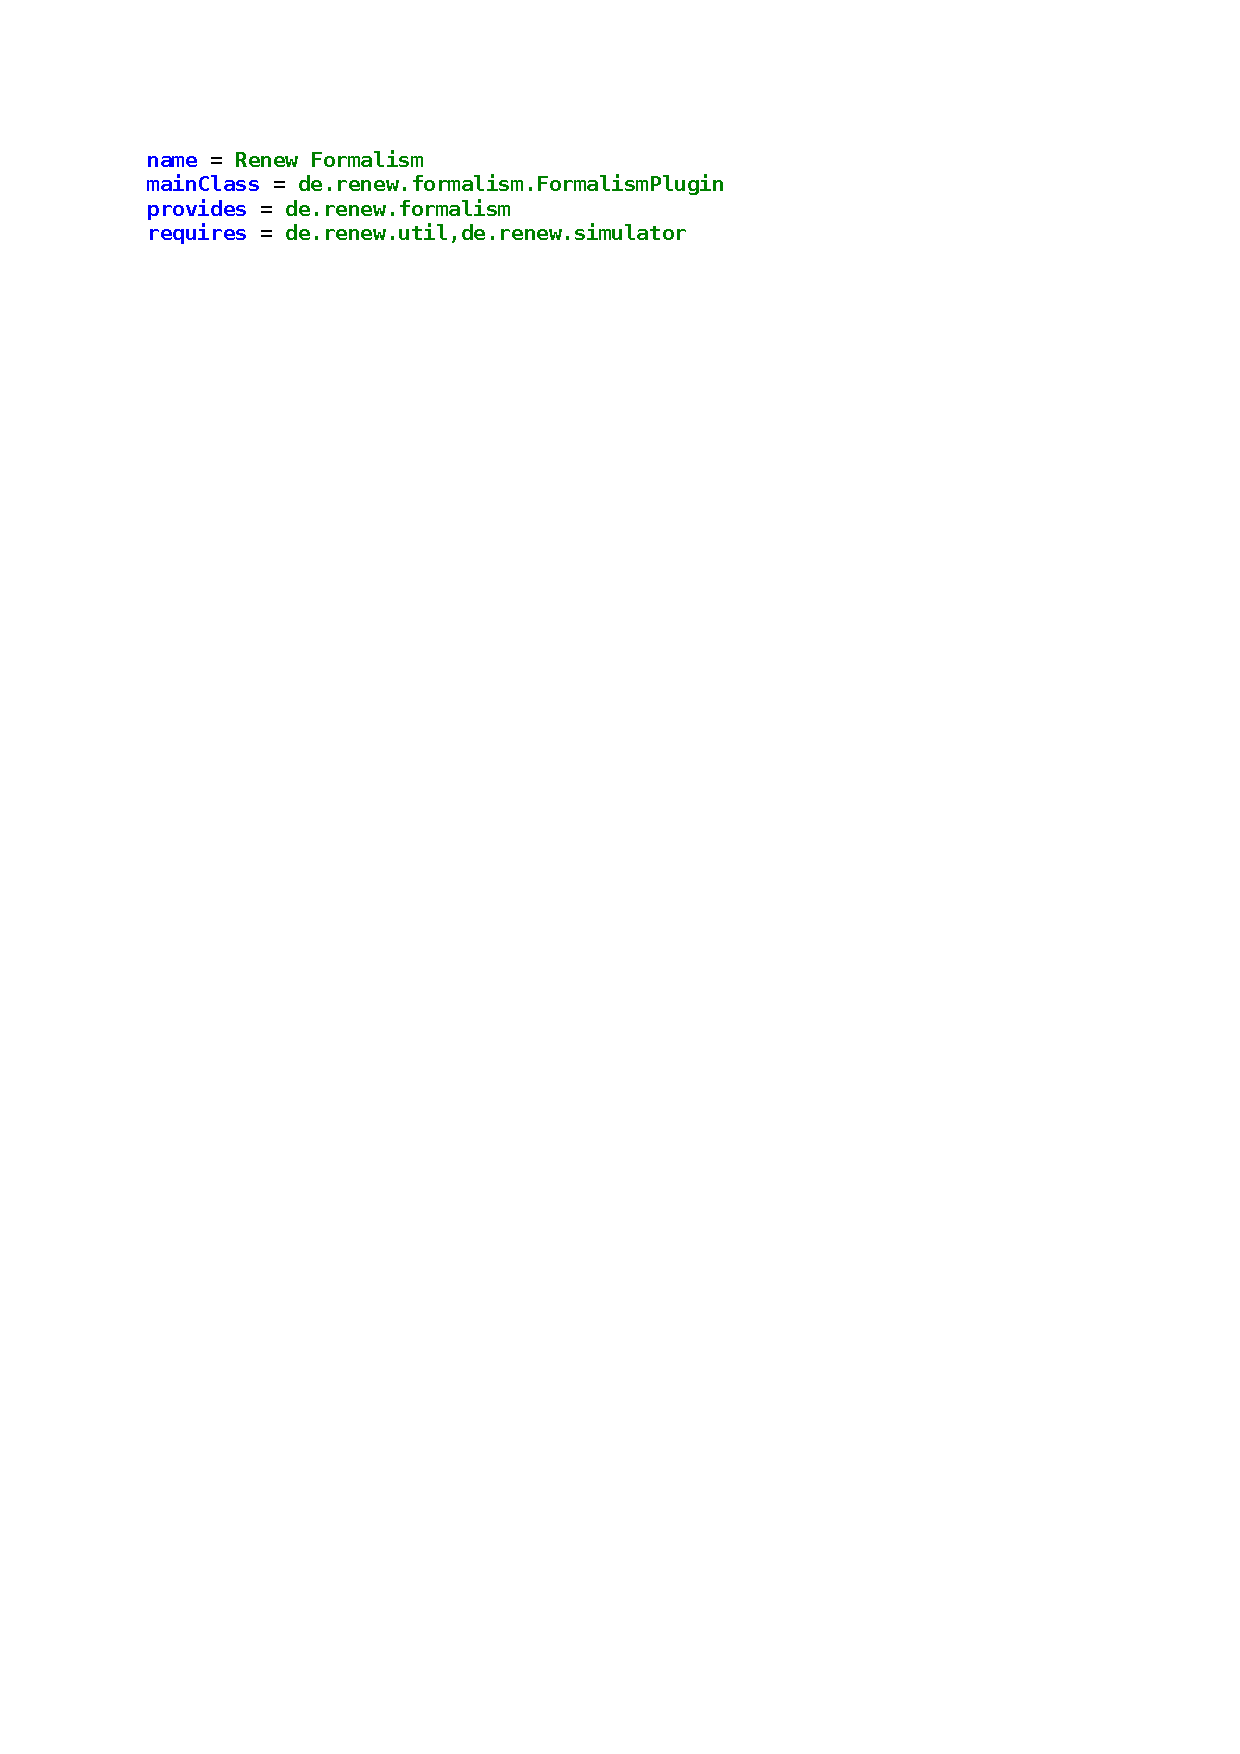
\includegraphics[width=0.6\textwidth]{material/images/cfg.pdf}
			  \caption{Die plugin.cfg}
			  \label{fig:plugin_cfg}
			\end{figure}
			% nachteil Drittanbieter werden nicht mitgezogen 
			Auch wenn die Plugin Abhängigkeit in der \textit{plugin.cfg} existieren, beinhalten die Konfigurationsdatei keine Drittanbieter-Bibliotheken, die ein wichtiger Bestandsteil der Software abbilden. In der Konsequenz kann \textsc{Renew} nicht automatisch nachprüfen, ob alle benötigten Drittanbieter-Bibliotheken integriert und mitgeliefert worden sind, um die Software für die Ausführung zu validieren.\newline
			% nachteile Homogene Umgebung
			Des Weiteren besitzt die \textit{plugin.cfg} ausschließlich der Information über die Laufzeitumgebung, die sich gegenüber der Entwicklungsumgebung unterscheiden kann. Denn die Entwickler arbeiten auf einer bestens eingerichteten Maschine mit allen nötigen Bibliotheken und Abhängigkeit, die in der Zielumgebung zu meist nicht existieren. Um der Diskrepanz des Ausführungskontextes entgegenzuwirken, wird eine Richtlinie benötigt, die den Kontext einer Applikation beschreibt. Leider wird dieses Verhalten nicht von der \textit{plugin.cfg} unterstützt. 

		\subsubsection{Die Stärken der module-info.java} \label{sub:module-info.java}
			%  problemstellung der module-info.java (das und dies war nicht toll und deswegen)
			Die Java Module wurden entwickelt, um die Codebasis beherrschbar, flexibel und austauschbar zu gestalten. Demzufolge verfolgt der Modularisierungsansatz und das Plugin Konzept eine ähnliche Herangehensweise. Der Modularisierungsansatz nutzt die \textit{module-info.java} Konfigurationsdatei, die die Information aus der \textit{plugin.cfg} aufgreift und erweitert. \newline
			\begin{figure}[h!]
			  \centering
			  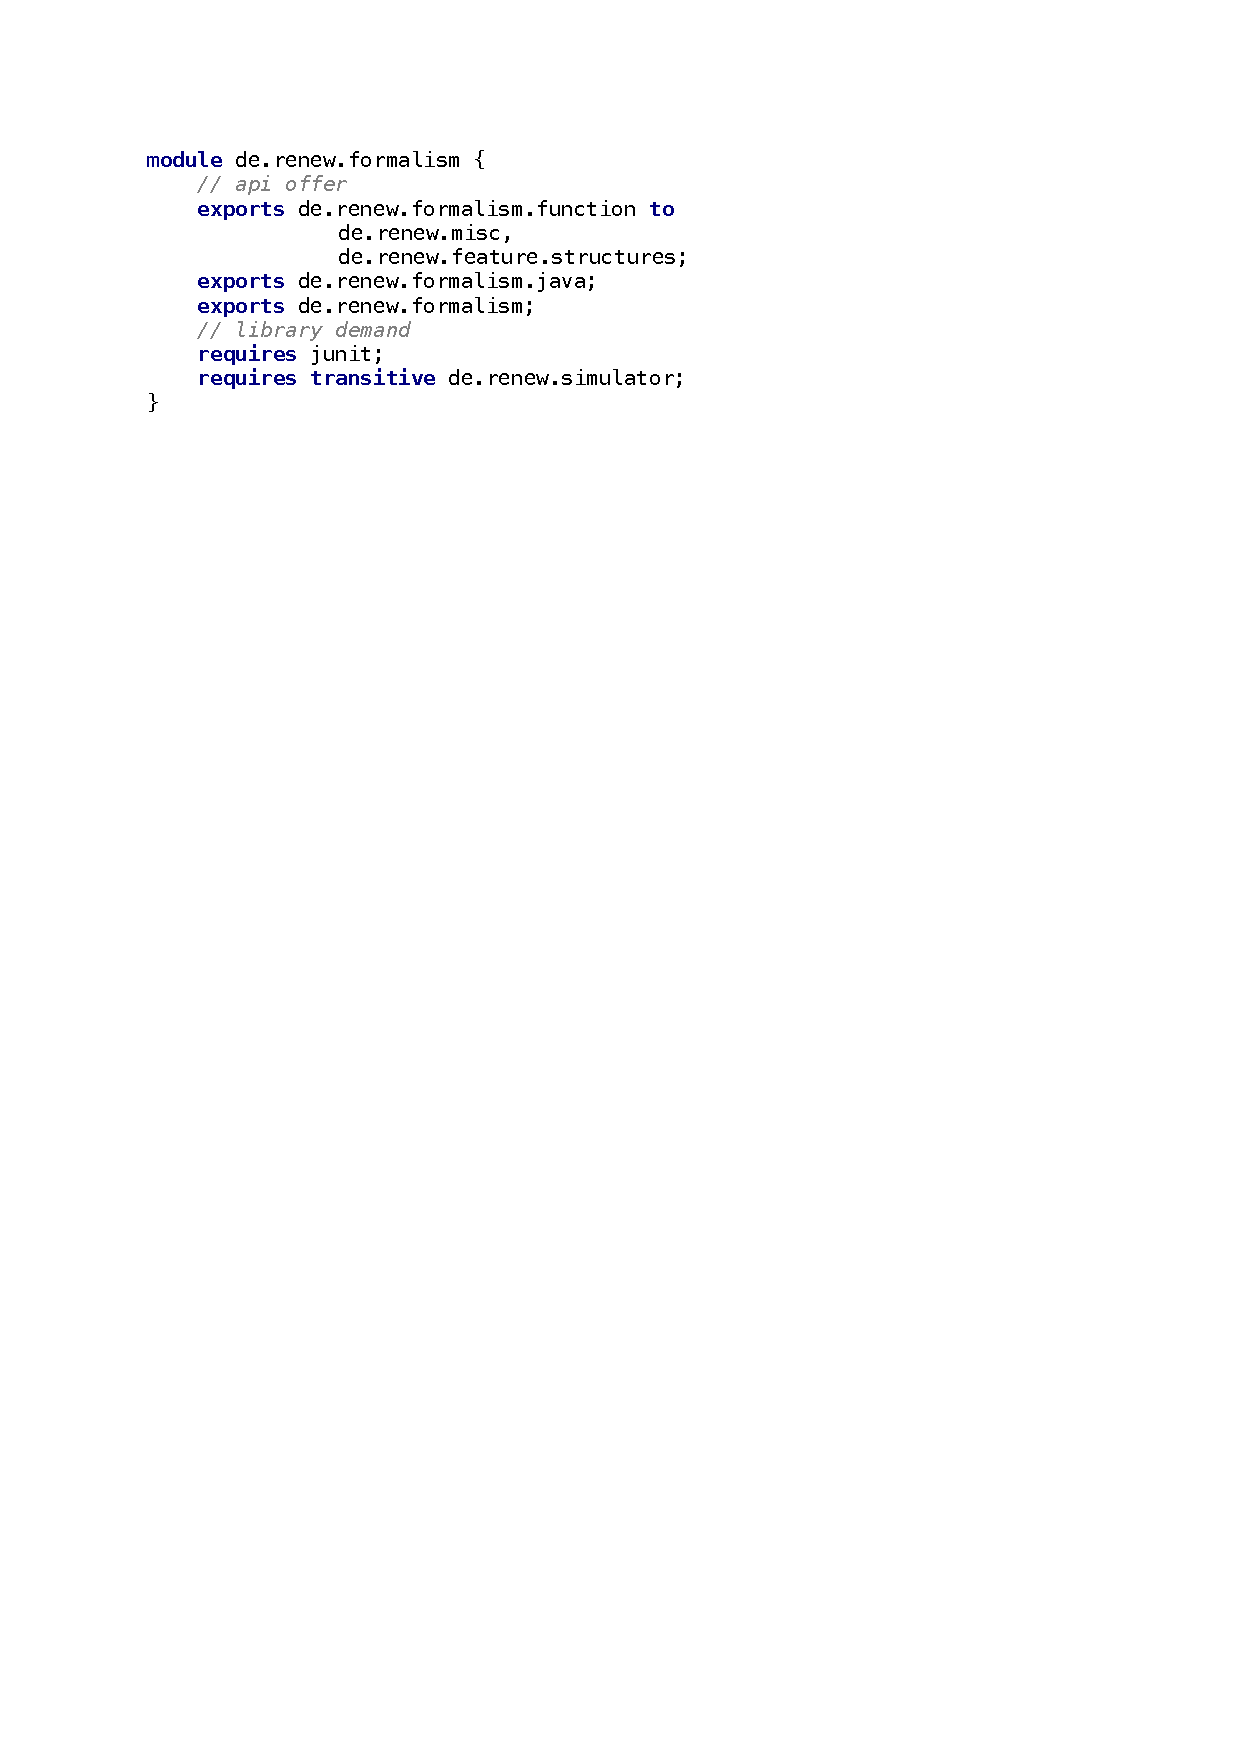
\includegraphics[width=0.6\textwidth]{material/images/m-info.pdf}
			  \caption{Die module-info.java}
			  \label{fig:module_info}
			\end{figure}

			Der Unterschied zwischen der \textit{module-info.java} und der \textit{plugin.cfg} wird bei der ersten Betrachtung sofort ersichtlich, denn die \textit{module-info.java} schränkt den Zugriffsraum auf das Modul ein, indem nur ausgewählte Schnittstellenpakete geöffnet werden, die darüber hinaus von jedem oder nur von auserwählten Konsumenten genutzt werden können. In der Abbildung \ref{fig:module_info} wird die Funktion des \textit{formalism} Plugins über das Paket \textit{de.renew.formalism.function} für die \textsc{Renew} \textit{misc} und \textit{feature structure} Plugins freigegeben. \newline
			Somit enthält jedes Plugin-Modul einen verpflichtenden Kommunikationsvertrag, mit dem das Modul mit seiner Umgebung kommuniziert.\newline
			Die verpflichtende Eigenschaft ist neu für \textit{Renew}, da die \textit{plugin.cfg} bislang nur eine optionale Beschriftung trägt und Fehler oder Mängel zu einem späten Zeitpunkt ungünstig auftreten lässt. Um dem entgegenzuwirken, greift Java direkt in das Projekt ein und führt die benötigten statischen Analysen durch, bevor die Applikation kompiliert und ausgeführt wird. Die Inspektion ist in Java integriert und stellt sicher, dass alle Abhängigkeiten zur Kompilations- sowie Laufzeit verfügbar sind und keine von diesen einen Zyklus hervorruft.\newline
			Die Validation mit der \textit{plugin.cfg} ist leider nicht möglich, da sie nicht Teil der Java Plattform ist und nur von dem \textsc{Renew} Plugin Manager zur Laufzeit verarbeitet wird. Des Weiteren unterstützt die \textit{module-info.java} transitive und statische Abhängigkeiten, die flexible Modul-Zugriffsrechte für die Nutzung weiterreichen und bestimmte Module für optional deklarieren. Dementsprechend wird der Kontext eines Plugin-Moduls implizit an seine Nutzer weitergereicht und macht das Lesen der benötigten Abhängigkeiten verständlich. Denn die explizite Deklaration jedes benötigten Plugin-Moduls und der dazugehörigen Drittanbieter-Bibliotheken, kann zu hunderten Einträgen führen, die an der Stelle keinen Beitrag zu der Struktur leisten. 

		\subsubsection{Direkter Vergleich} \label{sub:Direkter_Vergleich}
			Im Folgende wird eine Tabelle mit Eigenschaften abgebildet, die Gemeinsamkeiten und Unterschiede der beiden Konfigurationsdatei darstellt.\bigbreak
			% bild vergleich 
			\begin{table}[!h]
			\centering
			\begin{tabular}{l|l}
				\textbf{module-info.java} & \textbf{plugin.cfg} \\
				\hline
				\\[-1em]
				Plugin Abhängigkeiten & Plugin Abhängigkeiten \\
				\\[-1em]
			    Bibliothek Abhängigkeiten & \\
			    \\[-1em]
			    Entwicklung- und Laufzeitanalyse & Laufzeitanalyse \\
			    \\[-1em]
			    Wesentlich & Redundant \\
			    \\[-1em]
			    Funktonangebot & Codeangebot \\
			    \\[-1em]
			    Plattform Verpflichtend & Plattform Optional \\
			    \\[-1em]
			    Einschränkender Zugriff & Offener Zugriff \\
			    \\[-1em]
			    Gekapselt und Eindeutig & Gemischt und Verteilt \\
			    \\[-1em]
			    Integrierte Java Dienste & Renew Dienste \\
			    \\[-1em]
			    Namen & Namen \\
			    \\[-1em]
			    & Beschreibung \\
			    \\[-1em]
			    & Eigenschaften \\
			    \\[-1em]
			    & Version \\
			    \\[-1em]
			    & Einstiegspunkt
			    \\[-1em]
			\end{tabular}
			\end{table}

	\newpage
	
\section{Ausgangssituation} \label{sec:ausgangssituation} 
	In diesem Abschnitt wird die Ausgangssituation für \textsc{Renew} sowie \textsc{Mulan} dargelegt, die als Grundlage für die nachfolgenden Prototypen dienen werden. 

	\subsection{Renew Prototyp} \label{sub:renew}
		\textsc{Renew} ist in mehr als 60 Plugins aufgeteilt, die für sich alleinstehende Projekte repräsentieren. Jedes Projekt besitzt eine \textit{build.xml} und wird mit dem übergeordneten Stamm \textit{build.xml} Script zusammengeführt. Die XML-Scripte werden von dem \textit{Apach Ant} Werkzeug evaluiert, kompiliert und zusammengeführt. Infolgedessen entsteht ein \textit{jar} Archiv für jedes Plugin-Projekt. Diese werden in eine bestimmte Orderstruktur für die Ausführung aufbereitet, die sich aus dem \textit{config, plugins} und \textit{libs} Verzeichnis zusammensetzt. \bigbreak

		Der innere Aufbau jedes Plugins benötigt eine besondere Konfigurationsdatei, nämlich die \textit{plugin.cfg}. Diese beschreibt für die Ausführung nötigen Plugin-Abhängigkeiten und wird von dem internen Plugin-Manager verwaltet, der für die richtige Ordnung beim Laden jedes einzelnen Plugins aus dem \textit{plugins} Verzeichnis sorgt. Somit sind die \textit{plugin.cfg} Dokumente ein guter Startpunkt für die Evaluation einer minimalen und lauffähigen \textsc{Renew} Konfiguration. \bigbreak

		\begin{figure}[h!]
		  \centering
		  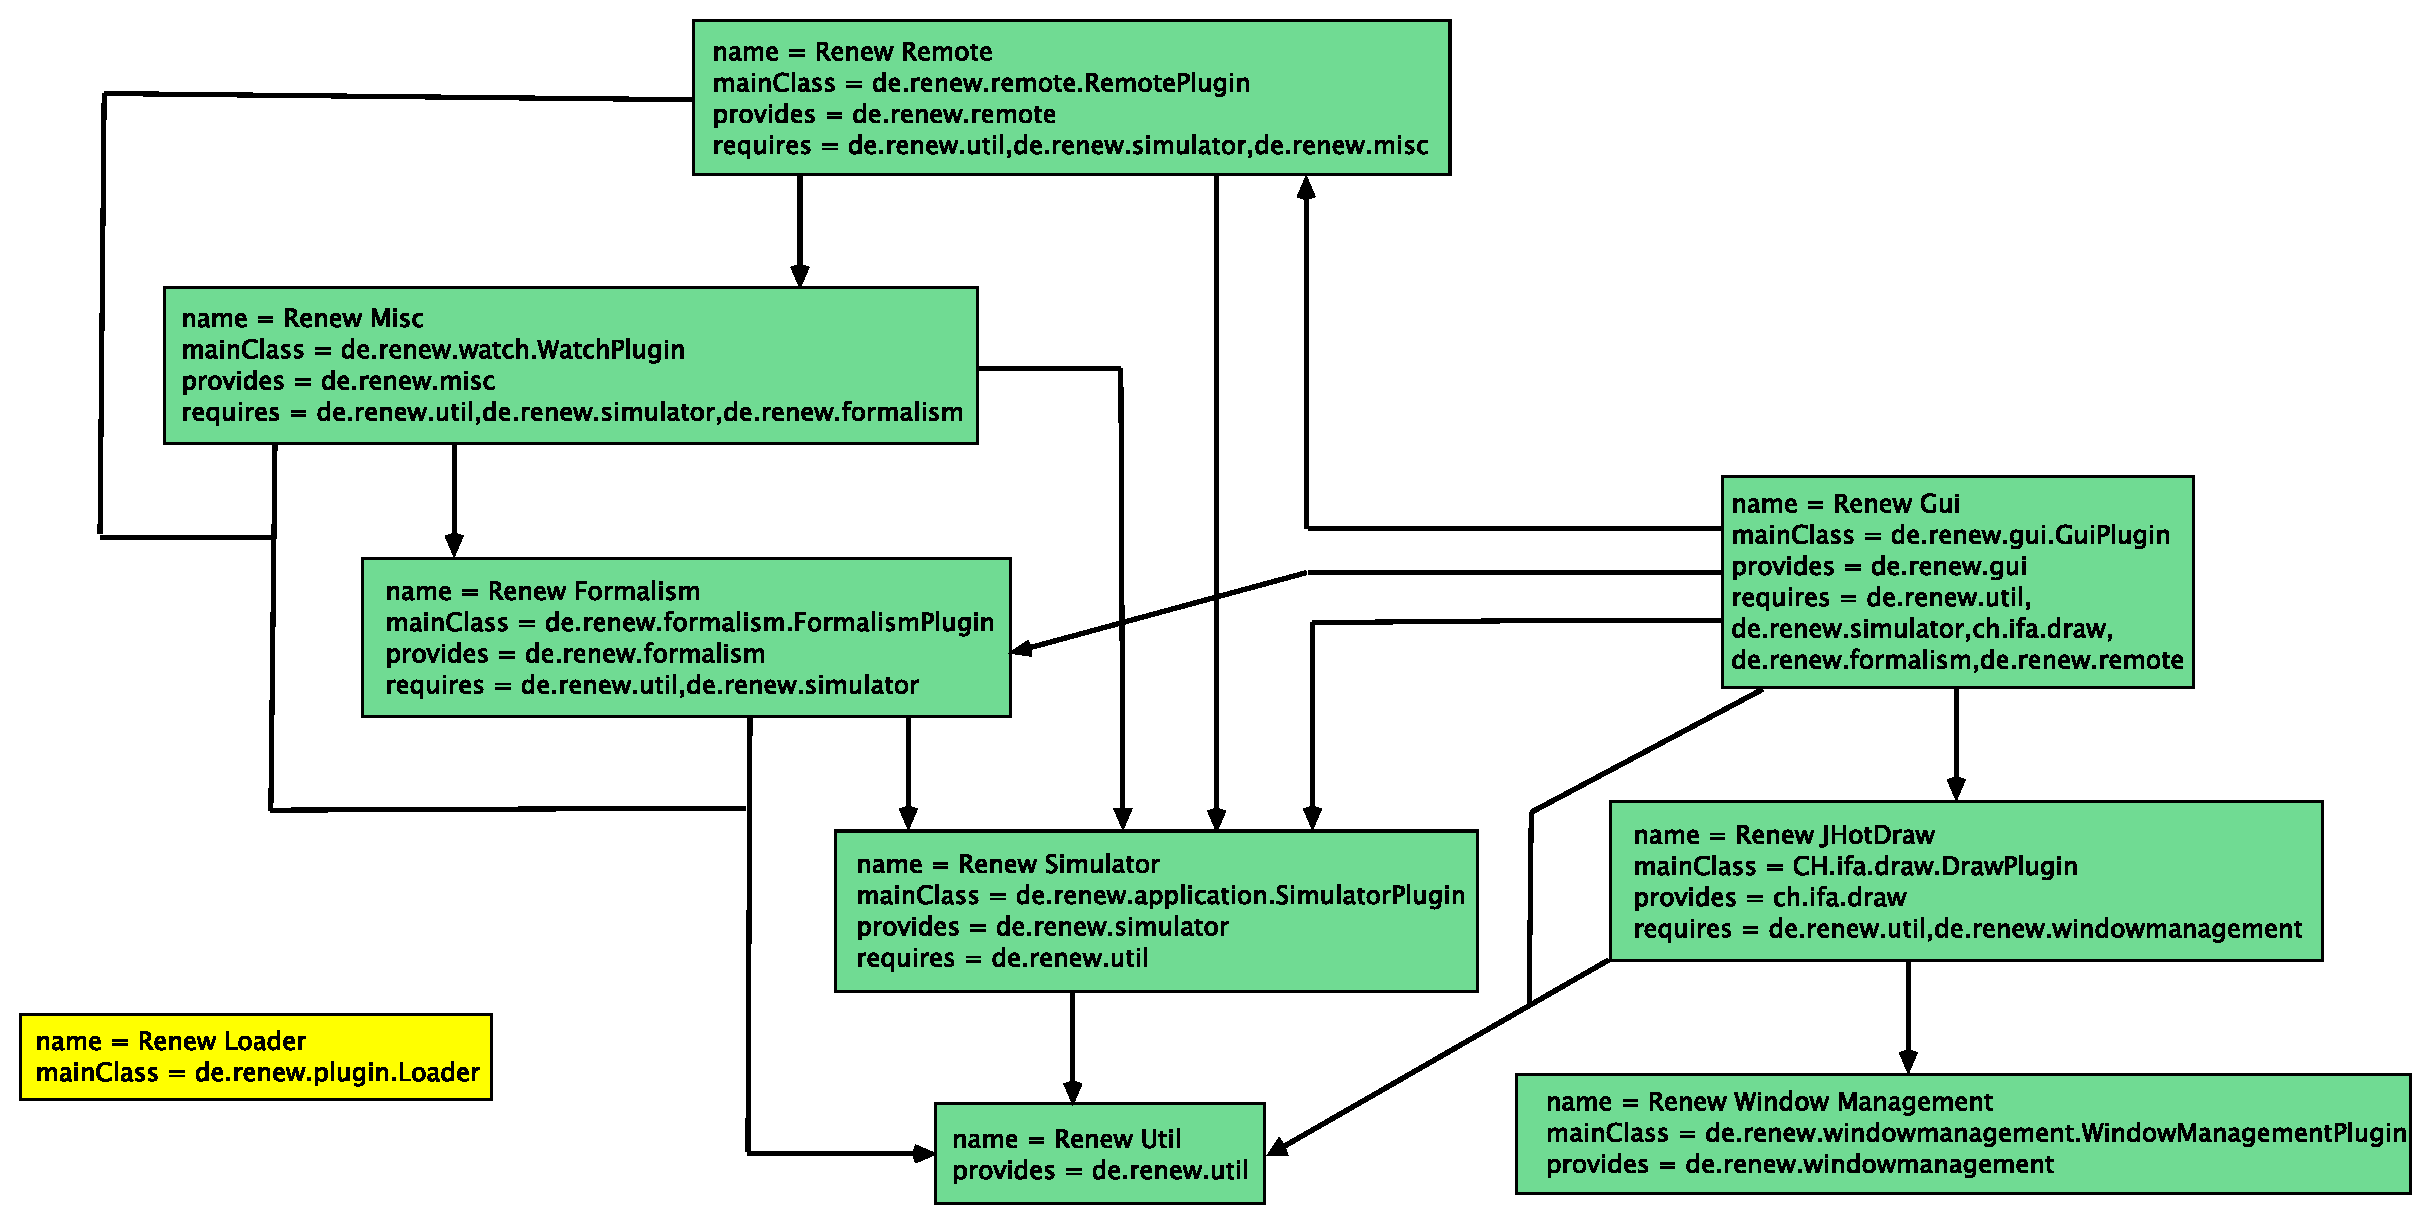
\includegraphics[scale=0.457, angle=90]{material/images/renew_plugin_dependencies2.pdf}
		  \caption{Gui Plugin-Abhängigkeiten}
		  \label{fig:plugin_deps}
		\end{figure}

		Für die Evaluation der minimalen Konfiguration starten wir aus dem \textit{Gui}-Plugin und arbeiten uns abwärts der Plugin-Hierarchie der \textit{plugin.cfg's} hinab, bis der komplette Graph aufgebaut ist. \newline

		Die in der Abbildung \ref{fig:plugin_deps} repräsentierten Zusammenhänge reflektieren die von den Entwicklern abgestimmten Laufzeitabhängigkeiten, die einen groben Überblick über die nötigen Plugins verschaffen. Diese können zur Laufzeit alle benötigten Daten und Klassen enthalten, jedoch tragen sie keine Aussage über Abhängigkeiten während der Kompilation. Demgemäß kann zusätzlicher Code sowie Plugins benötigt werden. 

	\subsection{Mulan Prototyp} \label{sub:mulan}
		\textsc{Mulan} \cite{Roelke04} ist ein Multi-Agenten-Rahmenwerk, mit dem Agenten entwickelt und miteinander verbunden werden können. Diese agieren nach eigenem Interesse und verhandeln über Kommunikationskanäle, die von \textsc{Mulan} angeboten werden. Um eine auf \textsc{Mulan} basierende Multi-Agent-Anwendung zu erstellen, müssen zahlreiche Protokollnetze gezeichnet und Wissensbasen erstellt werden, die das Verhalten und die Interaktion von Agenten implementieren. Somit bietet \textsc{Mulan} eine Kommunikationsplattform sowie ein Gerüst für die Umsetzung der darauf aufsetzenden Agenten und dessen Eigenschaften sowie Fähigkeiten, die mit Referenznetzen entworfen werden können. \cite{Cabac10a} \bigbreak

		Das Spiel Settler ist mit \textsc{Mulan} umgesetzt und implementiert somit die Agenten Anforderungen des Multi-Agenten-Systems. Diese halten Wissensbasen über die Spielregeln und können mithilfe der Protokollnetze bestimmte Entscheidungen treffen und Handlungen ausführen. Wie zum Beispiel Straßen bauen oder mit Karten handeln.\bigbreak
		
		\begin{figure}[h!]
		  \centering
		  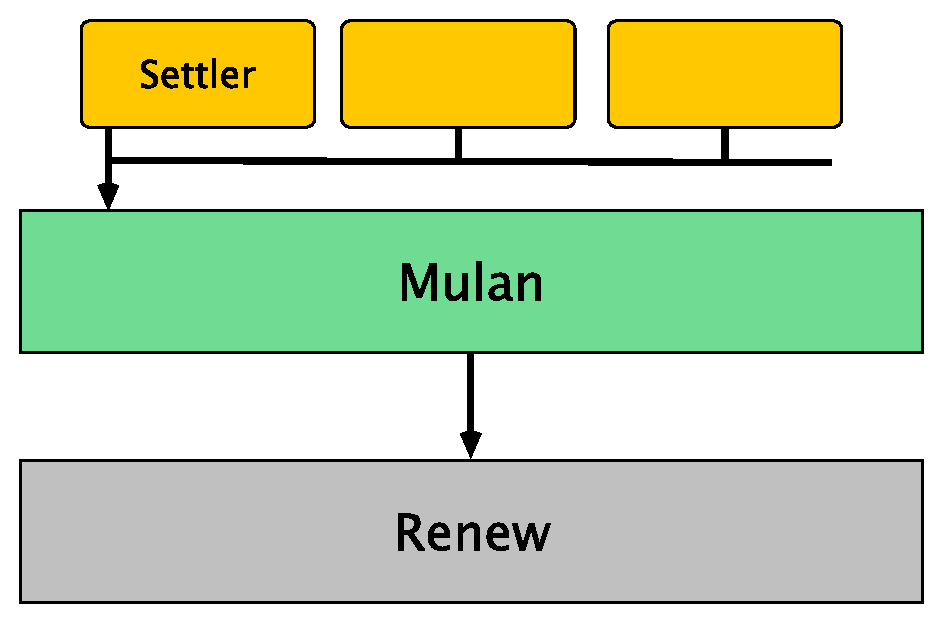
\includegraphics[width=0.5\textwidth]{material/images/settler-mulan-renew.pdf}
		  \caption{\textsc{Mulan} Plugins}
		  \label{fig:mulan_plugin}
		\end{figure}

		Damit die erstellten Settler Agenten und dessen Aufbau simuliert werden können, wird der \textsc{Renew} Petri-Netz Simulator verwendet, mit dem die umgesetzten Agenten-Strukturen betrieben werden können.\newline
		Des Weiteren besitzt das Settler Spiel sowie das \textsc{Mulan}-Rahmenwerk eine Plugin-konforme Architektur und werden somit genauso, wie die \textsc{Renew} Plugins von dem \textsc{Renew} Plugin-Manager ausgelesen und verwaltete.\bigbreak

		Ein vereinfachter Zusammenhang ist in der Abbildung \ref{fig:mulan_plugin} dargestellt und visualisiert die benötigten Grundlagen für die Ausführung von Settler.


	\subsection{Grundriss Prototyp} \label{sec:zustandRNW}
		Die Umsetzung der \textsc{Renew} Plugin-Architektur ist mit einem Klassenlader-System umgesetzt worden, welches den \textsc{Renew}-Code in drei Gruppen aufteilt und durch drei separate Klassenlader in die Applikation aufnimmt. Die Klassenlader verfolgen den empfohlenen und integrierten \textit{parent first} Ansatz, der in dem Kapitel \ref{sec:cls} diskutiert wurde und delegiert somit jede Anfrage zuerst an seinen übergeordneten Klassenlader, bevor die Klassensuche selbständig durchgeführt wird. \newline
		In der ersten Klassenlader-Instanz wird die Basis etabliert, die den Plugin-Manager sowie die Drittanbieter-Bibliotheken einliest und den darunterliegenden Plugin-Klassenlader mit Funktion versorgt. Der Plugin-Klassenlader lädt anschließend alle Plugins nacheinander in der richtigen Reihenfolge ein und garantiert zur Laufzeit das Vorkommen jeder benötigten Plugin-Klasse auf dem Klassenpfad. Zuletzt wird ein dynamischer Klassenlader erstellt, der für das Simulieren der Petri-Netze entsprechende Klassen und Ressourcen beim Ausführen einliest und nach der Simulation vergisst. \newline
		Die Umsetzung des Klassenlader-Systems von Michael Duvigneau wird in der Abbildung \ref{fig:classLoadDuv} dargestellt. \bigbreak
		% Bild Klassloader 
		\begin{figure}[h!]
		\centering
			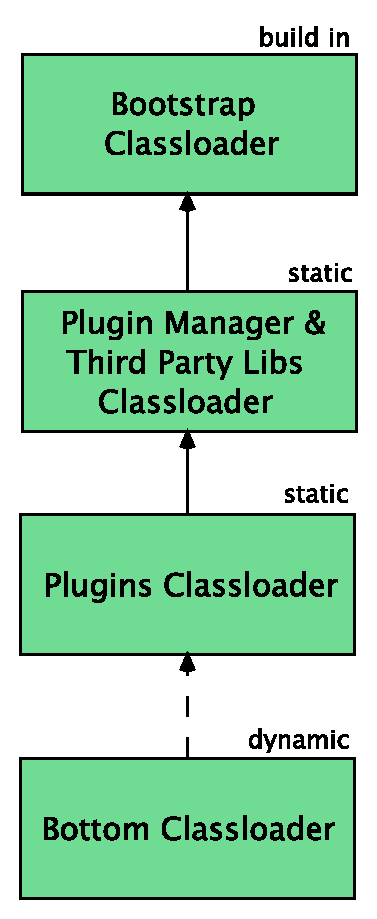
\includegraphics[width=0.3\textwidth]{material/images/Classloader-Hierarhie-Renew.pdf}
			\caption{\textsc{Renew} Klassenlader-System von Duvigneau \cite{Duvigneau09}}
			\label{fig:classLoadDuv}
		\end{figure}\bigbreak
		Duvigneaus Java Prototyp \cite{Duvigneau09} sollte eine Plugin-Verwaltung anbieten, die Plugins einfach sowie dynamisch neu konfigurieren lässt und das Hinzufügen und Entfernen von Plugins während der Laufzeit ermöglicht. Da der Prototyp nur die Praxistauglichkeit demonstrieren sollte, wurde eine \textit{schnelle} Variante implementiert, die nur die nötigste Funktionalität bereitstellt. Die Umsetzung der Klassenlader-Architektur aus der Abbildung \ref{fig:classLoadDuv} hat sich als ausreichend jedoch nicht mängelfrei herausgestellt. Die Umsetzung unterstützte ein essenzielles Charakteristikum eines dynamischen Systems nicht, nämlich das Entladen der Plugin-Codebasis aus der Applikation während der Laufzeit. Denn die Plugins werden mit einem gemeinsamen Klassenlader in das System eingebunden, der keine Möglichkeit anbietet eine auserwählte Codebasis zu vergessen. Dementsprechend können Plugins, die mit einem gemeinsamen Klassenlader geladen worden sind, nicht mehr separat behandelt werden. Dies hat zur Folge, dass die Applikation während der Laufzeit ständig wächst und die Möglichkeit verliert Plugins zu aktualisieren. Somit ist man an einen Neustart angewiesen, der die initiale Codebasis zurücksetzt und die Plugins entfernt oder aktualisiert. Daraus folgt eine erhebliche Beeinträchtigung der Wartbarkeit und der Systemstabilität für Systeme mit einem permanenten Betrieb. \bigbreak
		Einer der möglichen Lösungsansätze beschreibt das Erstellen eines Klassenlader per Plugin und die Aufbereitung sowie Verwaltung der Kommunikation zwischen diesen. Da der mitgelieferte Klassenlader von Java nur einen übergeordnet Klassenlader akzeptiert, erfordert die Umsetzung eine eigene Klassenlader-Implementation, die variable Eltern-Kontenmenge akzeptiert und die Delegation intelligent umsetzt. Jedoch ist die genannte Umsetzung aufwendig und benötigt viel Eigenimplementation. \newline
		Eine Alternative bietet das \textit{OSGi} Rahmenwerk, welches auf dynamische Systeme ausgelegt ist und eine Komponentenbasierte Entwicklung ermöglicht. Das \textit{OSGi} Rahmenwerk organisiert den Code in \textit{bundles}, die sich auf separaten \textit{OSGi} Klassenlader-Implementation befinden und über eine Verknüpfung der \textit{bundles} eine Applikation modellieren. \newline
		Die Umsetzung von \textit{OSGi} im \textsc{Renew} Kontext hat sich für schwierig erwiesen, da die Verwaltung der Plugins als \textit{OSGi bundles} mit einem erweiterten Lebenszyklus und Kommunikationsschwierigkeiten den gewünschten Anforderungen nicht entsprach \cite{Duvigneau09}. Demzufolge wurde die Java-Umsetzung des Klassenlader-Systems \ref{fig:classLoadDuv} der \textit{OSGi}-Umsetzung vorgezogen und bis zum jetzigen Zeitpunkt einwandfrei betrieben. \bigbreak

		Mit der Einführung des Modulsystems von Java, ist Java fähig das benannte Problem anzugehen und bietet eine Alternative zu den beiden genannten Lösungsansätzen. Die Umsetzungsmöglichkeit der dynamischen Plugin-Verwaltung wird im nächsten Abschnitt der neu eingeführten Modulschichten diskutiert. 


\section{Durchführung} \label{sec:durchführung}
	Die wichtigen Szenarien für das Erreichen des gesetzten Ziels werden mit drei Prototypen umgesetzt. Der \textsc{Renew} Prototyp wird eine kontinuierliche Modularisierung der Plugins und dessen Betriebsfähigkeit mit nur zum Teil Modularisierter Codebasis abdecken. Dazu gehört das Erstellen einer neuen Projektstruktur für die auserwählten Plugins und behandelt auserwählte Richtlinien, die mit dem Modulsystem von Java eingeführt worden sind. Für das Anfertigen von ausführbarem Code, wird das Gradle Werkzeug integriert, das einen Kompilation-Kontext für die neuen Module erstellt. Dazu gehört eine Abhängigkeitsverwaltung sowie Projektkopplung. Um die Plugins mit einender als Module zu verzahnen, werden Schnittstellen untersucht und in der \textit{module-info} Konfigurationsdatei in den Plugins verankert. In der folgenden Evaluation wird das Ergebnis evaluiert und sauber aufbereitet.\bigbreak 

	Im Gegensatz dazu behandelt der \textsc{Mulan} Prototyp die Zusammenführung bestehender Systeme mit modularisiertem Code. Für die Umsetzung werden nur für das Spiel Settler relevanten \textsc{Mulan} Plugins erarbeitet und auf die minimale \textsc{Renew} Version aufgesetzt. Doch zuerst muss eine erweiterte Analyse der minimalen \textsc{Renew} Version durchgeführt werden, um die benötigten \textsc{Renew} Plugins für das \textsc{Mulan} Rahmenwerk nachzurüsten. Im weiteren Verlauf behandelt dieser Prototyp Konsequenzen der Umstellung auf eine neue \textsc{Renew} Grundlage und der benötigten Ausführungsschritte für die Adaption. Die Evaluation bewertet den Aufwand für die Umsetzung des Prototyps. \bigbreak

	Zum Schluss erforscht der \textit{Grundriss}-Prototyp das Modulschichtenkonzept und modelliert eine mögliche Umsetzung des Plugin-Systems, das Plugins separat betreiben und ausführen kann. Des Weiteren wird das Konzept des \textit{Service-Laders} integriert und soll die Plugins als Dienste in die Software eingliedern, die entkoppelt voneinander betrieben werden können. \newline
	Der \textit{Grundriss}-Prototyp wird keine Logik von \textit{Renew} oder \textit{Mulan} beinhalten und soll nur den möglichen Einsatz der neuen Technologien demonstrieren. \newline
	Abschließend wird der Prototyp untersucht und auf Mängel sowie unerwartetes Verhalten evaluiert.


